\documentclass{standalone}
\usepackage{tikz}
\usetikzlibrary{intersections}

\tikzset{align at bottom/.style={baseline=(current bounding box.south)}}

\begin{document}
	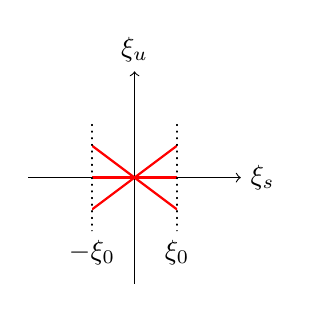
\begin{tikzpicture}[scale = 0.27]
	
		\draw[->] (-5, 0) -- (5, 0);
		\draw[->] (0, -5) -- (0, 5);
		\node[right] at (5, 0) {$\xi_s$};
		\node[above] at (0, 5) {$\xi_u$};
		
		%\draw[draw = black, fill = gray, fill opacity = 0.2, draw opacity = 0.5, name path = support_cut_off] (-4, 0) -- (-1.5, 3) -- (1.5, 3) -- (4, 0) -- (1.5, -3) -- (-1.5, -3) -- cycle;
		
		\begin{scope}
		
			\clip (-2, -2) rectangle (2, 2);
			
			\draw[red, thick, cap = round] (-2, 1.5) -- (2, -1.5);
			\draw[red, thick, cap = round] (-2, 0) -- (2, 0);
			\draw[red, thick, cap = round] (-2, -1.5) -- (2, 1.5);
			
		\end{scope}
		
		\draw[black, cap = round, dotted] (-2, 2.5) -- (-2, -2.5);
		\draw[black, cap = round, dotted] (2, 2.5) -- (2, -2.5);
		
		\node[below] at (-2, -2.5) {$-\xi_0$};
		\node[below] at (2, -2.5) {$\xi_0$};
		
	\end{tikzpicture}
	
\end{document}